\documentclass[a4paper]{article}

\usepackage{INTERSPEECH2019}
\usepackage{amsmath,graphicx}
\usepackage{amssymb}
\usepackage{mathtools}
\DeclareMathOperator*{\argmin}{\min}
\usepackage{tikz}
\usepackage{adjustbox}
\usepackage{enumitem}
\usepackage{tikz-cd}
\usepackage{makecell}%
\usepackage{pgfplots}
\usepackage{pgfplotstable}
\usepackage{filecontents}
\usepackage{tkz-euclide}
\usepackage{setspace}
\usepackage{blkarray}
\newcommand*\rot{\rotatebox{90}}
\newcommand*\OK{\ding{51}}
\usepackage{multirow} 
\usepackage{hhline}
\usepackage{threeparttable}
\usepackage{subfig}
\usepackage[noadjust]{cite}
%\usepackage{cite}
%\doublespacing
\usetikzlibrary{pgfplots.dateplot}
\usetikzlibrary{matrix,decorations.pathreplacing,fit,calc,positioning,chains}
\tikzset{ 
	table/.style={
		matrix of math nodes,
		row sep=-0.5ex,
		column sep=-0.5ex,
		nodes={rectangle,text width=3em,align=center},
		text depth=1.25ex,
		text height=2.5ex,
		nodes in empty cells,
		%left delimiter=[,
		%right delimiter={]},
		ampersand replacement=\&		
	}
}

\tikzset{%
	highlight1/.style={rectangle,rounded corners,color=black!,fill=blue!15,draw,fill opacity=0.5,thick,inner sep=0pt}
}

% Example definitions.
% --------------------
\def\x{{\mathbf x}}
\def\L{{\cal L}}
\title{Comparative Study of Text Representation 
	Methods For Subjectivity Analysis}
\name{names}
%The maximum number of authors in the author list is twenty. If the number of contributing authors is more than twenty, they should be listed in a footnote or in acknowledgement section, as appropriate.
\address{
	Dept. of CSE, Manipal Institute of Technology Karnataka, Manipal, India, 576 104}
\email{email}

\begin{document}

\maketitle
% 
\begin{abstract}
  With the advent of contextual word-embeddings like ELMo and BERT, the sphe
  This paper compares several representations of text within the same experimental setting for subjectivity analysis. The representations compared in this paper are the traditional N-gram, bag-of-words (BoW) model, followed by word embeddings like Word2Vec and GloVe. 
  
   
\end{abstract}
\noindent\textbf{Index Terms}: Natural Language Processing(NLP)

\section{Introduction}
\label{sec:intro}

Natural Language Processing (NLP) is the study of interaction between computers and humans using the natural language.. It has many emerging applications such as; machine translation \cite{stork2012audio}, speech recognition \cite{goetze2012acoustic}, audio surveillance \cite{foggia2015reliable} \cite{mulimani2019extraction}, machine hearing \cite{lyon2010machine} and so on.


\section{Text Representation Methods}
\label{sec:format}
 The process of transforming text into numeric stuff, is usually performed by building a language model. These models typically assign probabilities, frequencies or some obscure numbers to words, sequences of words, group of words, section of documents or whole documents. The language models implemented in this paper are explained below in brief.

\subsection{N-gram Language Model}

\subsection{Bag-of-words Language Model}
\subsection{N-gram Language Model}
\subsection{Word2vec language model}
\subsection{Glove language model}




















%In this step, we extract the SIFT feature vectors from the grayscale Gammatonegram $GI(f, t)$. 
David G. Lowe, first introduced the SIFT algorithm for object recognition in a digital image \cite{lowe2004distinctive}. SIFT algorithm includes two main stages: keypoint detection and feature extraction. Algorithm first localizes (detects) interesting keypoints in the grayscale Gammatonegram of an acoustic event (see blue color keypoints in Fig.~\ref{fig2}) and the second stage extracts a set of 128-dimensional feature vectors associated with detected keypoints for VFs representations using LLC. 
\begin{figure}[!t]
	
	\centerline{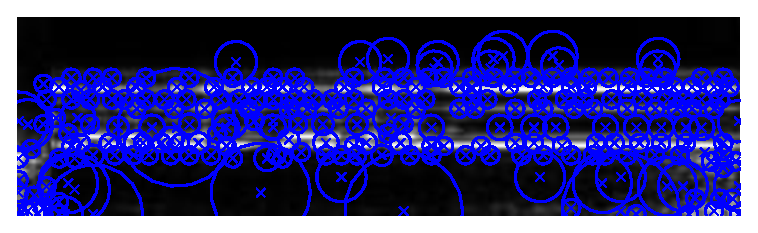
\includegraphics[width=8cm,height=2.3cm]{g34}}
	
	\caption{SIFT keypoints of acoustic event ringing phone.}
	\label{fig2}
	%
\end{figure}
\subsection{Visual vocabulary generation}
Let $Y$ be a set of $D$-dimensional feature vectors (row vectors or SIFT vectors) extracted from a grayscale Gammatonegram, i.e., $Y=[y_1,  y_2,...,y_N] \in \mathbb{R}^{N\times D}$.  A set of feature vectors $Y$ of five randomly selected acoustic events per class are grouped into mutually exclusive clusters using the K-means clustering algorithm.  The centroids of these clusters are referred to as visual words or codewords.  All the visual words together constitute a
vocabulary $V$ or a codebook. It is worth to point out that five acoustic events per class are sufficient enough to build discriminative visual vocabulary with less computational time. There is no known best way to select
the size of the vocabulary $M$, i.e., the number of visual words. In
this work, the size of the vocabulary ranging from 64 to 512
is considered and its impact on the performance of AEC is
analyzed.
\subsection{Locality-constrained Linear Coding}
Given a set of D-dimensional feature vectors $Y$ (row vectors or SIFT) from a grayscale  Gammatonegram and a vocabulary $V$ with $M$ entries, $V=[v_1,  v_2,...,v_M] \in \mathbb{R}^{M\times D}$, Locality-constrained Linear Coding (LLC) converts each feature vector into a $M$-dimensional code for AEC \cite{wang2010locality}. The objective function of LLC is formulated as:
\begin{equation}
\begin{multlined}
\argmin\limits_{C}\sum_{i=1}^{N}\|y_i-Vc_i\|^2+\lambda\|d_i\odot c_i\|^2\\
s.t.\; 1^Tc_i=1, \forall i \;\;\;\;\;\;\;\;\;\;\;\;\;\;\;\;\;\;\;\;\;\;\;\;\;\;\;\;\;\;\;\;\;
\end{multlined}
\label{eq2}
\end{equation}
Where $C=[c_1, c_2,..., c_N]$ is a set of coding coefficients (codes) for $Y$, $\odot$ represents the element-wise multiplication, $d_i\in \mathbb{R}^N$ is a distance vector (evaluated using Euclidean distance) between $y_i$ and each visual word of the vocabulary $V$, $\lambda$ is a regularization parameter, which weights the locality constraint.

Minimizing the Eq. (\ref{eq2}) tends to encode each feature vector $y_i \in Y$ into a $M$-dimensional code using visual words of vocabulary $V$. Locality adaptor $d_i$ penalizes the visual words far away from the feature vector. 
Specifically, a larger $d_i$ suppresses the value of corresponding code $c_i$ to zero. 
Hence, the resulting set of codes $C \in \mathbb{R}^{N\times M}$ is a sparse representation of $Y$ with few non-zero elements. It can also be interpreted as each feature vector $y_i \in Y$ only responses to nearby visual words of vocabulary $V$. 
\subsection{Visual feature vector generation}
In this step, a single $M$-dimensional code $Z=[z_1,z_2,...,z_M]\in \mathbb{R}^{1\times M}$ is obtained from the set of codes  $C$ (the result of Eq. (\ref{eq2})) using max pooling function $Z=max(C)$. Specifically, a maximum value is chosen from $C$ in a column-wise manner as given in (\ref{eq3}).
\begin{equation}
z_j=max\{c_{1j},c_{2j},...,c_{Nj}\}
\label{eq3}
\end{equation}
Where N is number of feature vectors in $Y$.
Each column  of $C$ corresponds to the responses of all feature vectors in $Y$ to a visual word in $V.$ 

The pooled features ($Z$) are also known as codes of visual features, which are normalized using $\ell_2$ norm. Normalized visual features of row vectors and SIFT vectors of grayscale Gammatonegram are fused (concatenated) to get Fused Visual Features (FVFs). 
\label{sec:typestyle}
\begin{table*}[ht]
	\caption{Comparison of overall Recognition accuracy (\%) of proposed FVFs with other methods at clean and different SNR conditions on UPC-TALP and DCASE datasets. }
	\scriptsize
	\begin{center}
		\begin{tabular}{|c|c|c|c|c|c|c||c|c|c|c|c|}
			\hline
			\multicolumn{2}{|c|}{} &	\multicolumn{5}{c||}{UPC-TALP}&\multicolumn{5}{c|}{DCASE}\\
			\hline
			Method & \makecell{Ref.}& \makecell{Clean}&\makecell{20dB}& \makecell{10dB}& 0dB & Average & Clean & 20dB & 10dB & 0dB & Average\\
			\hline
			\hline
			MFCCs &-& 74.79& 66.46&58.55&46.88&61.67&50.94& 43.68&38.44&26.93&39.99\\
			\hline
			GTCCs		&\cite{valero2012gammatone} &{76.87} & 74.83& 72.54 & 59.02 & 70.81 &{54.06} & 51.25& 48.13 & 37.75 & 47.79 \\
			\hline
			DNNs &\cite{kong2016deep}& 70.42 & 69.38 & 58.55 & 35.63&58.49& 39.69 & 38.12 & 33.44 & 25.00&34.07\\
			\hline
			CNNs&\cite{li2017comparison}& 86.33 & 84.05 & 80.17 & 65.97&79.13& 65.25 & 61.30 & 57.17 & 45.32&57.26\\
			\hline
			BoVW &\cite{mulimani2018robust}& {93.54} & {92.51} & {88.76} & {79.54} &{88.58}& {68.75} & {66.25} & {59.37} & {46.88} &{60.31}\\
			\hline
			SIFT vectors - VFs &-& {94.06} & {92.96} & {90.21} & {80.71} &{89.48}&{75.01} & {70.63} & {61.57} & {47.19} &{63.06}\\
			\hline
			Row vectors - VFs &-& {95.01} & {93.34} & {92.30} & {86.26} &{91.72}& {79.07} & {74.34} & {65.63} & {53.76} &{68.02}\\
			\hline
			FVFs &-& \textbf{99.17} & \textbf{99.15} & \textbf{98.12} & \textbf{89.17} &\textbf{96.40}& \textbf{96.32} & \textbf{93.19} & \textbf{90.69} & \textbf{81.63} &\textbf{90.45}\\
			\hline
		\end{tabular}
	\end{center}
	\label{table1}
\end{table*}   
\section{Experiments}
\label{sec:pagestyle}
\subsection{Acoustic event datasets}
Performance of the proposed approach is evaluated using two publicly available datasets namely UPC-TALP dataset \cite{temko2006clear} and DCASE-2013 dataset \cite{stowell2015detection}. 
\subsubsection{UPC-TALP dataset}
A 12 different isolated meeting room acoustic events, namely: applause,  chair moving, cough, door knock, door slam, keyboard typing, key jingle, laugh, paper wrapping, phone ring, spoon cup jingle and steps are selected for AEC. Approximately 60 acoustic events per class, recorded using 84 microphones, namely: an array of 64 Mark III microphones, 12 T-shape clusters microphones, 8 table top and omni-directional microphones are used. In this work, only the third channel of Mark III array is considered for the experiments. 
\subsubsection{DCASE dataset}
A 16 different isolated acoustic events namely, alert, clearing throat, cough, door slam, drawer, keyboard, keys, knock, laugh, mouse, page-turn, pen drop, phone ring, printer, speech and switch are used for AEC.  Approximately 27 acoustic events per class are presented in the DCASE dataset. In this work, microphone channel one from stereo recordings is considered for the performance evaluation.

Acoustic events of both the datasets are trimmed to the length of given annotations and resulting data is divided into five disjoint folds to perform five-fold cross-validation. Each fold has the equal number of acoustic events per class. 
To compare the robustness of the proposed approach, 'speech babble' noise from NOISEX'92 database \cite{varga1993assessment} is added to the acoustic events at 20, 10 and 0dB SNR. The 'speech babble' noise is diffuse and most of its energy is distributed at lower frequencies. All acoustic events are processed at 44100 Hz sampling rate.
\subsection{Evaluation methods}
Performance of the proposed approach is compared with the following baseline system and the other state-of-the-art methods of AEC.
\begin{enumerate}
	\item Baseline system : Mean and standard deviation of 13 MFCCs and their first and second-order derivatives are taken over each frame, resulting in $39\times2$ dimensional feature vector. 
	\item GTCCs : Mean and standard deviation of 13  Gammatone Cepstral Coefficients (GTCCs) and their first and second-order derivatives are taken over each frame \cite{valero2012gammatone}, resulting in $39\times2$ dimensional feature vector. 
	\item DNNs : Mel band energies are used as features to DNNs, which has three fully connected layers followed by a softmax output. Each layer uses 500 units with ReLU activation function and 10\% dropout. Categorical cross-entropy used as a loss function \cite{kong2016deep}. 
	\item CNNs : 60-dimensional log Mel features used as input features to 
	Convolutional Neural Networks (CNN).
	%, which has layers architecture similar to VGG net \cite{simonyan2014very}. 
	The network had two CNN's of 32, 64 and 128 filters. Each CNN is followed by batch-normalization and Rectified Linear Unit (ReLU). CNN's with same number filters followed by max pooling.   A softmax activation function is used as the output layer \cite{li2017comparison}.
	\item BoVW : Grayscale spectrograms of acoustic events are represented as BoVW \cite{mulimani2018robust} features to train Chi-square kernel SVM for AEC.
\end{enumerate}
The MFCC and GTCC features used in our experiments are extracted using 20ms hamming window with 50\% overlap and normalized to zero mean and unit variance. Results of all the methods except DNNs, CNNs and BoVW are reported using linear kernel SVM, which achieves higher recognition accuracy with lower computation cost. %hence, it is chosen as a classifier.
Hence, one-versus-rest multi-class SVM is chosen as a classifier and its  optimal parameters (such as C) are selected using five-fold cross-validation. 
%The five-fold cross-validation is performed to select optimal parameters of one-versus-rest multi-class SVM.
%One-versus-rest multi-class SVM is trained with five-fold cross-validation.
\section{Results and Discussion}
%\begin{table}
%	\scriptsize
%	\centering
%	\caption{Comparison of overall Recognition accuracy (\%) of proposed SIFT-based BoVW approach with other methods using Chi-square SVM at clean and different SNR.}
%	\begin{tabular}{|c|c|c|c|c|c|}
%		\hline
%		Method & Clean &20dB &10dB &0dB & Average\\
%		\hline
%		\hline
%	Gammatonegram - VFs & {95.01} & {93.34} & {92.30} & {86.26} &{91.72}\\
%	\hline
%	Spectrogram - VFs & {90.63} & {88.55} & {83.34} & {68.75} &{82.81}\\
%	\hline
%		Spectrogram SIFT - VFs & {93.96} & {91.46} & {90.21} & {81.71} &{89.33}\\
%		\hline
%		Gammatonegram SIFT - VFs & {91.68} & {90.63} & {89.17} & {81.28} &{88.19}\\
%		\hline
%	
%	\end{tabular}
%	
%	\label{table2}
%\end{table}
%\begin{table}
%	\scriptsize
%	\centering
%	\caption{Comparison of overall Recognition accuracy (\%) of proposed FVFs with other methods using linear SVM at clean and different SNR conditions on UPC-TALP dataset.}
%	\begin{tabular}{|c|c|c|c|c|c|c|}
%		\hline
%		Method & Ref. & Clean &20dB &10dB &0dB & Average\\
%		\hline
%		% 		Bark & 75 & 21.75&10.96\\
%		% 		\hline
%		% 		MFCC & 80.25 &19& 5.48\\
%		\hline
%		MFCCs &-& 74.79& 66.46&58.55&46.88&61.67\\
%		\hline
%		%	\multirow{3}{*}	{MFCC-BoAW} &Linear &87.08 & 82.51& 77.51 & 50.84 & 74.48 \\
%		%		\hhline{~------}
%		%		&Intersection &{88.76} & 86.68& 81.05 & 56.67 & 78.39 \\
%		%		\hhline{~------}
%		GTCCs		&\cite{valero2012gammatone} &{76.87} & 74.83& 72.54 & 59.02 & 70.81 \\
%		\hline
%		%	\multirow{3}{*}	{MFCC-BoAW} &Linear &87.08 & 82.51& 77.51 & 50.84 & 74.48 \\
%		%		\hhline{~------}
%		%		&Intersection &{88.76} & 86.68& 81.05 & 56.67 & 78.39 \\
%		%		\hhline{~------}
%		
%		DNNs &\cite{kong2016deep}& 70.42 & 69.38 & 58.55 & 35.63&58.49\\
%		\hline
%		CNNs&\cite{li2017comparison}& 86.33 & 84.05 & 80.17 & 65.97&79.13\\
%		\hline
%		BoVW &\cite{mulimani2018robust}& {93.54} & {92.51} & {88.76} & {79.54} &{88.58}\\
%		\hline
%		%	MFCC-BoAW &Chi-square& 66.67 & 60.63 & 55.22 & 37.51 &55.00\\
%		%	\hline
%		%	SIF-SVM &Chi-square& 76.67 & 75.84 & 74.17 & 60.84&71.88\\
%		%	\hline 
%		%Foggia et al. &\cite{foggia2015reliable}& 88.34 & 85.42 & 76.46 & 62.09&78.07\\
%		%\hline 
%		SIFT vectors - VFs &-& {94.06} & {92.96} & {90.21} & {80.71} &{89.48}\\
%		\hline
%		Row vectors - VFs &-& {95.01} & {93.34} & {92.30} & {86.26} &{91.72}\\
%		\hline
%		FVFs &-& \textbf{99.17} & \textbf{99.15} & \textbf{98.12} & \textbf{89.17} &\textbf{96.40}\\
%		\hline
%	\end{tabular}
%	
%	\label{table1}
%\end{table}
%\begin{figure}
%	\pgfplotstableread[row sep=\\,col sep=&]{
%		interval & carT & carD & carR\\
%		clean     & 93.96  & 95.01  & 99.17\\
%		20dB	&91.46 & 93.34 & 99.15\\
%		10dB & 90.21 & 92.30 & 98.12\\
%	0dB     & 81.71 & 86.26  & 89.17\\
%	Avg. & 89.33 & 91.72 &96.40\\
%	}\mydata
%	\begin{tikzpicture}
%	\begin{axis}[
%	ybar,
%	%x=7cm,
%	bar width=.2cm,
%	width=9cm,
%	height=5.5cm,
%	enlarge x limits={abs=1.1cm},
%	legend style={at={(0.52,0.37)},
%		anchor=north east,legend columns=1},
%	symbolic x coords={clean,20dB,10dB,0dB,Avg.},
%	xtick=data,
%	%nodes near coords,
%	%nodes near coords align={vertical},
%	ymin=80,ymax=100,
%	ylabel={Accuracy (\%)},
%	]
%	\addplot table[x=interval,y=carT]{\mydata};
%	\addplot table[x=interval,y=carD]{\mydata};
%	\addplot table[x=interval,y=carR]{\mydata};
%	%\addplot table[x=interval,y=FFV]{\mydata};
%	\legend{Gammatonegram VFs, SIFT VFs, FVFs}
%	\end{axis}
%	\end{tikzpicture}
%	\caption{Recognition accuracy of Red, Green, Blue and Fusion Fisher Vectors at clean and 0dB SNR.}
%	\label{fig4}
%\end{figure}
The experimental results given in Table~\ref{table1} demonstrate that proposed FVFs-SVM combination significantly outperforms all the methods in clean and different noisy conditions with average recognition accuracy of 96.40\% and 90.45\% on UPC-TALP and DCASE datasets, respectively. The recognition performance of all the methods on DCASE dataset is lower compared to performance on UPC-TALP dataset. This is due to the quality of DCASE audio recordings, which are already quite noisy (there are no clean acoustic events) and real SNR might be lower than denoted. Hence, the performance of all the methods drastically reduces in clean and noisy conditions. However, the proposed FVFs discriminate acoustic events from the noise and largely outperform all other methods in clean and noisy conditions.

As we had mentioned earlier, the speech babble noise is diffuse and its maximum energy concentrated at lower frequencies. The MFCCs are sensitive to noise at lower frequencies. Hence, the performance of the MFCCs baseline system significantly drops at 0dB SNR.

The GTCCs are also obtained from Gammatone filter bank as our grayscale Gammatonegram. Hence, GTCCs are considered for performance comparison with FVFs in this
work. Gammatone filterbank resolution at lower frequencies
is much higher with ERB scale than Mel filter bank with Mel
scale. Hence, GTCCs discriminate the spectral components at lower frequencies belong to the acoustic event and
noise accurately than MFCCs. However, the performance of
GTCCs still worse when compared to proposed FVFs.

Further, the performance of FVFs-SVM combination is also compared with the emerging DNNs and CNNs. The CNNs are effective and outperform DNNs in clean and noisy conditions (see Table~\ref{table1}). However, CNNs/DNNs require huge data for training and do not perform very well in the cases of limited training data.  

Our previous BoVW approach \cite{mulimani2018robust} performs significantly better in clean and noisy conditions. However, BoVWs are the histograms of traditional VQ codes obtained from Grayscale spectrograms of acoustic events. In VQ, similar (nearby) feature vectors of acoustic events have different VQ codes due to large quantization errors, in contrast to that of LLC which ensures similar LLC codes for the nearby feature vectors of the acoustic events.   Hence, LLC codes or VFs from row vectors and SIFT vectors of Gammatonegram significantly discriminate acoustic events in clean and noisy conditions than VQ codes.  It is worth to point out that, proposed VFs achieve impressive recognition accuracy with linear SVM. The BoVW approach performs well with non-linear kernel classifiers such as Intersection and Chi-square kernels SVMs, which demand higher computational time than simple linear SVM. 

The magnitude of the intensity values of an acoustic event in
the grayscale Gammatonegram is much higher than that of noise. The
noise is distributed over Gammatonegram compared to the acoustic
event and its maximum energy is concentrated at the lower region of Gammatonegram. However, higher intensity values (strongest peaks) of the acoustic events are unaffected by noise (see Fig.~\ref{fig:res} at clean and 0dB SNR), which are effectively
discriminated by VFs (row vector VFs) in all noisy conditions. 

The SIFT feature extraction algorithm blurs the grayscale Gammatonegrams using different scales before keypoint localization that highlights the strongest peaks of the acoustic events and reduces the effect of noise. Further, localizes the keypoints around the strongest peaks of an acoustic event and extracts the SIFT feature vectors from detected keypoints. Hence, VFs from SIFT feature vectors of grayscale Gammatonegrams are robust to noise and outperform the BoVW in different noisy conditions.

However, VFs from row vectors or SIFT feature vectors does not perform alone as expected. The FVFs are the combination of significant VFs from row vectors and SIFT vectors of the Gammatonegram. Hence, the
FVFs contains significantly much more information about the acoustic events than VFs alone and they are observed to outperform all other approaches in both clean and noisy conditions.
\subsection{Recognition accuracy versus size of the codebook} 
The acoustic event recognition accuracy of
VFs from row vectors and SIFT vectors of Gammatonegrams with linear SVM to the number of visual words
i.e., size of the vocabulary at clean condition on UPC-TALP dataset is shown in
Fig.~\ref{fig9}. One can observe that recognition accuracy improves as
there is an increase in the number of visual words. The smaller
vocabulary groups the dissimilar acoustic events into the same
visual word. Hence, the smaller vocabulary is not much discriminative
and gives poor performance. On the other hand, the larger
vocabulary is more discriminative and achieves improved performance for both VFs. However, as the size of the vocabulary increases
computational complexity also increases. In this work, we
use 256 visual words (i.e., the size of the vocabulary) which generate
256-dimensional VFs from row and SIFT vectors for AEC with
higher recognition accuracy and lower computational cost. 
Further, both 256-dimensional VFs are concatenated to get 512-dimensional FVFs used for AEC.

\begin{figure}
	%	\centering
	\begin{filecontents}{div.data}
		M			 		Acc			Acc1
		10					67.71		56.25
		20					69.01		80.21
		30					81.25		82.29
		40					85.42		84.25
		50					92.71		88.55
		60					95.01		93.96
		70					95.35		93.98
		
	\end{filecontents}
	\begin{tikzpicture}
	\begin{axis}[
	%title={Temperature dependence of CuSO$_4\cdot$5H$_2$O solubility},
	width=8.5cm,
	height=3.8cm,
	y label style={at={(axis description cs:0.07,.5)}},
	xlabel style={align=center},
	legend style={at={(0.72,0.45)},
		anchor=north,legend columns=1},
	xlabel={Visual words},
	ylabel={Accuracy (\%)},
	xtick=data,
	xticklabels={8,16,32,64,128,256,512},
	ymin=50,ymax=100,
	xmin=10,xmax=70,
	xmajorgrids=true,
	ymajorgrids=true,
	grid style=dashed,
	]
	\addplot table[x=M,y=Acc] {div.data};
	\addplot table[x=M,y=Acc1] {div.data};
	\legend{Row vectors - VFs, SIFT vectors - VFs}
	\end{axis}
	\end{tikzpicture}
	\caption{Recognition accuracy versus number of visual words.}
	\label{fig9}
\end{figure} 
\subsection{Performance of the FVFs versus state-of-the-art methods on UPC-TALP and DCASE datasets}
The overall recognition accuracy of the FVFs at clean condition on UPC-TALP and DCASE datasets is also compared with the state-of-the-art methods reported in the literature (see Table~\ref{table2}). 
The traditional speech features are represented as BoAW in \cite{phan2016learn} and achieves 96.80\% of acoustic event recognition accuracy, which is less than that using proposed FVFs (i.e., 99.17\%) in clean condition, for UPC-TALP dataset. However, these speech features are sensitive to noise and performance of their BoAW representations is expected to reduce in noisy conditions. 
The effect of FVFs is clearly observed on DCASE dataset and it largely outperforms state-of-the-art HMM-based methods \cite{schroder2015spectro} \cite{jayalakshmi2018global}, which are also based on traditional speech features, may not be suitable for AEC.   
%\subsection{Results on DCASE dataset}
\begin{table}
	\scriptsize
	\centering
	\caption{Confusion matrix of all categories over the UNSW-NB15 dataset using Early Fusion classifier.}
	\begin{tabular}{|c|c|c|c|}
		\hline
		Dataset & Method & Ref. &Accuracy\\
		\hline
		% 		Bark & 75 & 21.75&10.96\\
		% 		\hline
		% 		MFCC & 80.25 &19& 5.48\\
		\hline
	UPC-TALP & BoAW - SVM& \cite{phan2016learn} & 96.80 \\
		\hline
	UPC-TALP & \makecell{Proposed\\ FVFs - SVM} & - & \textbf{99.17} \\
	\hline	
	\hline
	DCASE & \makecell{Gabor Filterbank \\ Features - HMM} & \cite{schroder2015spectro} & 80.00 \\
	\hline
	DCASE & \makecell{Global statistical \\ Features - HMM} & \cite{jayalakshmi2018global} & 70.31 \\
	\hline
		DCASE & \makecell{Proposed\\ FVFs -SVM} & - & \textbf{96.32} \\
		\hline	
	\end{tabular}
	
	\label{table2}
\end{table}
\section{Conclusions}
\label{sec:majhead}

In this paper, a novel FVFs are proposed for AEC.
FVFs are the combination of significant VFs, obtained from
row vectors and SIFT vectors of grayscale Gammatonegram of an acoustic event. Intensity values of the acoustic event in the grayscale Gammatonegram are higher than that of noise and those are effectively discriminated by FVFs.
FVFs achieve overall 96.40\% recognition accuracy in
clean and different noisy conditions. It indicates that proposed
FVFs features are robust and have a significant contribution
towards the AEC. In future, the concatenation of spectral
and other image features to FVFs may further improve
the performance of the proposed approach.

\section{Acknowledgements}
The authors would like to thank Ministry of Electronics \& Information Technology (MeitY), Government of India for their support in part of the research.


\bibliographystyle{IEEEtran}

\bibliography{mybib2}

%\begin{thebibliography}{9}

% \bibitem[1]{Davis80-COP}
%   S.\ B.\ Davis and P.\ Mermelstein,
%   ``Comparison of parametric representation for monosyllabic word recognition in continuously spoken sentences,''
%   \textit{IEEE Transactions on Acoustics, Speech and Signal Processing}, vol.~28, no.~4, pp.~357--366, 1980.
% \bibitem[2]{Rabiner89-ATO}
%   L.\ R.\ Rabiner,
%   ``A tutorial on hidden Markov models and selected applications in speech recognition,''
%   \textit{Proceedings of the IEEE}, vol.~77, no.~2, pp.~257-286, 1989.
% \bibitem[3]{Hastie09-TEO}
%   T.\ Hastie, R.\ Tibshirani, and J.\ Friedman,
%   \textit{The Elements of Statistical Learning -- Data Mining, Inference, and Prediction}.
%   New York: Springer, 2009.
% \bibitem[4]{YourName17-XXX}
%   F.\ Lastname1, F.\ Lastname2, and F.\ Lastname3,
%   ``Title of your INTERSPEECH 2019 publication,''
%   in \textit{Interspeech 2019 -- 20\textsuperscript{th} Annual Conference of the International Speech Communication Association, September 15-19, Graz, Austria, Proceedings, Proceedings}, 2019, pp.~100--104.
% \end{thebibliography}

\end{document}
